%% This is an example first chapter.  You should put chapter/appendix that you
%% write into a separate file, and add a line \include{yourfilename} to
%% main.tex, where `yourfilename.tex' is the name of the chapter/appendix file.
%% You can process specific files by typing their names in at the 
%% \files=
%% prompt when you run the file main.tex through LaTeX.
\chapter{Realizace}

Vlastní realizace struktury není pouhé vygenerování dat pomocí standartních dostupných nastavení, ovšem brzy bude, následný tisk, případný post-processing, a aplikace.

Jelikož se vlastnosti zejména vodivých filamentů zásadně liší od běžně dostupných, je patrné, že bude nutno proces dostatečně upravit pro úspěšné dokončení tisku, jeho opakovatelnosti a následné použitelnosti produktu. Podobně jako v případě post-processingu v podobě pokovení.

Naopak anténní čočka a vzorky pro extrakci parametrů lze realizovat standartním způsobem a je pouze otázkou časové náročnosti procesu a voblou správného materiálu.

\section{3D tisk}
Realizace veškerých struktur v této práci byla pomocí technologie 3D tisku FDM, kterou jsme si již vysvětlili v kapitole 1. Opět však je možnost zvolit nepřeberné množství tirkáren kterou jsou čím dál více dostupné, v tomto případě se jednalo o Original Prusa i3 MK2. Toto zařízení patří mezi nejpoužívanější stolní 3D tiskárny na světě \cite{3Dhubs} a existuje široká škála již před připravených, řádně otestovaných, tiskových nastavení ze které výrazně urychlí případné ladění pro specifický materiál.

\subsubsection{Trychtýřová anténa}
Jelikož bylo primárním cílem možnost použití produktu přímo bez post-processignu, je tedy nezbytné volit vodivé filamenty. Tyto materiály, jak již víme mají výrazně odlišné vlastnosti od jejich nosičů.

Pro námi navrženou anténu byly použity následující filamenty:
\begin{itemize}
\item Electrifi Conductive 3D Printing Filament
\item F-Electric Filament
\item Blackmagic 3D Conductive Graphene Filament
\item MKF Filament MKF-ABS F1.75 černá / VODIVÁ
\end{itemize}

Veškeré použité filamenty jsou na nosiči PLA, s vyjímkou MKF-ABS. Jako příměs jsou použity grafenové fragmenty (Blackmagic), uhlíkové nanotrubky (F-electric) a měďěné částice (Electrifi). Bohužel u materiálu MKF nebylo možné s dostatečnou přesností určit příměs jelikož výrobce tento údajneposkytuje. Podobná situace poté však ale platí i procentuální podíl příměsí, které jsou buďto tajné, či neznámé pro všechny testované vzorky.

Z hlediska vodivosti, tedy nejlepšího kandidáta na použití při realizaci dle udávaných parametrů (byly-li dostupné) je jednoznažně Electrify, který udává $16667\,S/m$. Nicméně je velmi důležitá jeho náročnost na tiskový proces vlivem velkého procenta mědi, která akumuluje teplo a značně prodlužuje zchlazení objektu pod teplotu skelného přechodu způsobující následnou deformaci tisknutého produktu vlivem gravitace.

Dalším významným faktorem filamenty Electrifi je jeho cena, $199.53\,CZK$/m. Pokud bychom tedy chtěli realizovat námi navržený trychtýř, bylo by nezbytné použít téměř 27\,m, celkem tedy $5 387\,CZK$ za předpokladu 100\,\% úspěšnosti realizace.

Jako reálnější materiály poté vychází F-electric, s vodivostí $133.33\,S/m$ a cenou $25.73\,CZK$/m, $694.71\,CZK$ za trychtýř, či Blackmagic, s vodivostí $166.67\,S$ a cenou $43.2\,CZK$/m, $1 166.4\,CZK$ za trychtýř, které vykazují výrazně vhodnější parametry pro tisk.

Před vlastní generací dat je však nutno vyrvořit profil charakterizující materiál z hlediska teplot, rychlosti procesu, chalzení, a ostatních parametrů. Pro získání prvnotního návrhu nastavení lze pouze převzít doporučené hodnoty výrobcem, nicméně ne vždy toto musí platit! Jelikož neexistuje jednotný standart pro 3D tiskrány typu: tiskový povrch, geometrie trysky, mechanika extruderu, a další, bude pravděpodobné že toto nastavení ve finální podobě bude odlišné.

\begin{figure}[h]
\begin{center}
\includegraphics[width=9.5cm]{pics/HornFinal}
\caption{Výsledný model trychtýřové antény včetně příruby na vlnovod realizovaný technologií 3D tisku za použití F-electric filamentu}
\label{fig:HornRealFe}
\end{center}
\end{figure}

Bohužel však při realizaci dalších struktur docházelo k významným komplikacím znemožňující další produkci, zejména k ucpavání trysky \ref{fig:HornFail}.

K těmto skutečnostem pravděpodobně vedlo nadměrné hromadění příměsí v místě zužení trysky způsobující zúst mechanického odporu a nároků na potřebnou sílu k jeho překonání. Vlivem nízké mechanické soudržnosti materiálu a křehkosti způsobeno vysokým procentem plnění poté dochází k prokluzování podávacího mechanismu extruderu a následného výpadku extruze. Další pravděpodobnou příčinou mohl být vlastní průměr filamentu, který pokud je mimo specifikaci ($\pm0.05\,mm$) může dojít k podobné situaci jelikož ne vždy je možné protáhnout předmět větší než rozměry otvoru. 

Tyto komplikace byly částečně eliminovány použitím trysky $D_{nozzle} = 0.6\,mm$, avšak problémy stále přetrvávali a proces byl velmi nespolehlivý a neopakovatelný. Možné další principy eliminace mohou být realizovány například úpravou mechanické části extruderu, která by měla výrazně větší styčnou plochu podávacího mechanismu s filamentem pro možnost vyvinou vyšší tlačnou sílu.

\begin{figure}[h]
\begin{center}
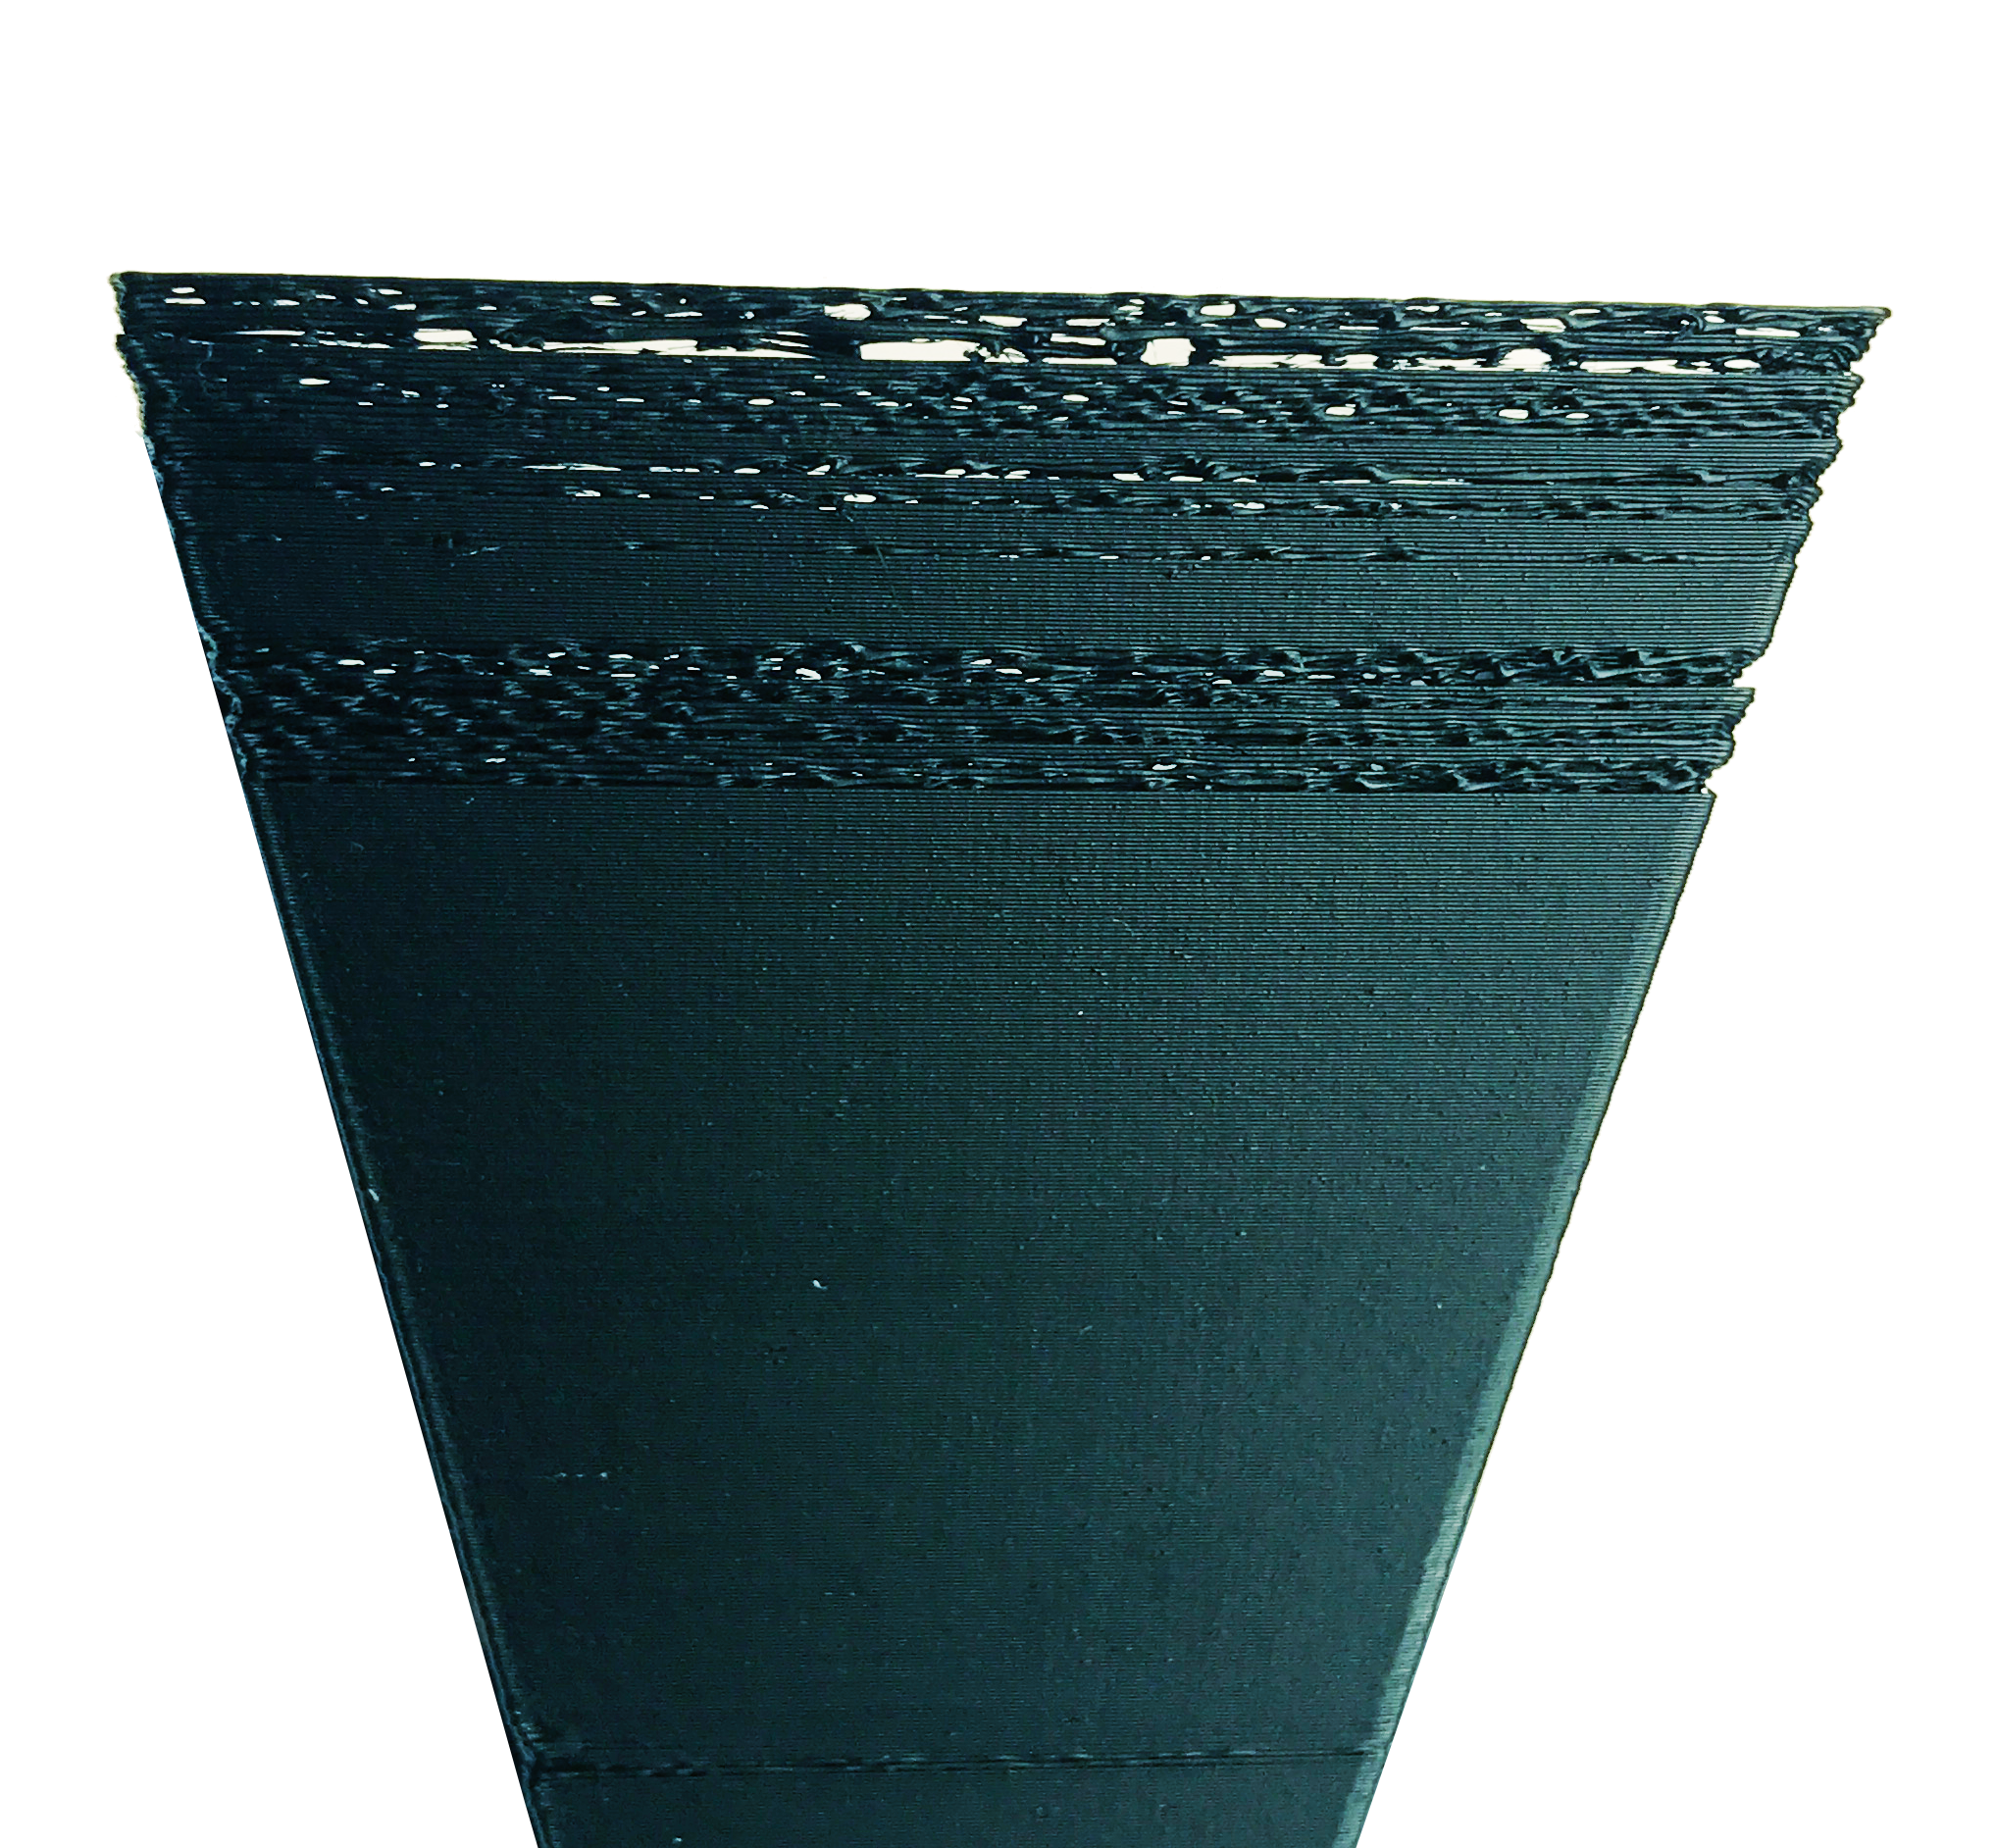
\includegraphics[width=9.5cm]{pics/HornFail}
\caption{Důsledek ucpavání trysky v průběhu tisku modelu}
\label{fig:HornFail}
\end{center}
\end{figure}


\subsubsection{Anténní čočka}
Realizace anténní čočky je v porovnání s předchozím případem velmi zjednodušena z důvodu zvolení zpomalujícího typu, tedy použití dielektrického, nikoliv vodivého, materiálu.

Pro správnou funkci čočky a maximálnímu přiblížení se simulovaných modelů je důležité při generování dat pro technologický proces použít správný typ vnitřní struktury pro zajištění 100\.\% podílu dielektrického materiálu.

Pokud toto nebude při realizaci dodrženo, vlivem nehomogenního prostředí pro šíření vlny, obsahující mnoho velmi ostrých rozhraní vzduch/dielektrikum, způsobí velmi odlišné chování a pro jeho dostatečný popis je třeba k téro struktuře přistupovat jako k metamateriálu.



\section{Pokovení}



\section{Měření parametrů}

\begin{figure}
\begin{tikzpicture}[scale=1.4]
\begin{axis}[
    xlabel={Angle /\,$^\circ$},
    ylabel={Amplitude /\,dB},
    minor tick num=10,
    minor grid style={gray!25},
  	major grid style={black!50},
  	xmin=-180,xmax = 180,
  	ymin=-120, ymax=-60,
    grid=both
]
\addplot [no markers, thick, blue] table [col sep=tab, y=Ae-graph] {horn.dat};
\addplot [no markers, thick, red] table [col sep=tab, y=Ae-emi] {horn.dat};
\addplot [no markers, thick, green] table [col sep=tab, y=Ae-lens] {horn.dat};
\end{axis}
\end{tikzpicture}
\caption{Řez naměřené vyzařovací charakteristiky realizovaného trychtýře z materiálu F-electric v E rovině}
\end{figure}

\begin{figure}
\begin{tikzpicture}
\begin{axis}[
    xlabel={Angle /\,$^\circ$},
    ylabel={Amplitude /\,dB},
    minor tick num=10,
    minor grid style={gray!25},
  	major grid style={black!50},
  	xmin=-180,xmax = 180,
  	ymin=-120, ymax=-60,
    grid=both
]
\addplot [no markers, thick, blue] table [col sep=tab, y=Ah-graph] {horn.dat};
\addplot [no markers, thick, red] table [col sep=tab, y=Ah-emi] {horn.dat};
\addplot [no markers, thick, green] table [col sep=tab, y=Ah-lens] {horn.dat};
\end{axis}
\end{tikzpicture}
\caption{Řez vyzařovací charakteristiky v H rovině}
\end{figure}



